\documentclass[12pt,a4paper,t,xcolor=dvipsnames,slidestop,compress,mathserif]{beamer}
\usepackage{amsmath,amssymb,graphicx,color,multicol,amsfonts,algorithmic,url,stmaryrd,epsf}
\usepackage{graphicx, algorithm}

%% ----------------------------------------------------------------------
%% Definitions, Macros, Etc.
%% ----------------------------------------------------------------------

%% Hyper-linked References
\newcommand{\Sec}[1]{\hyperref[sec:#1]{\S\ref*{sec:#1}}} %section
\newcommand{\Eqn}[1]{\hyperref[eq:#1]{(\ref*{eq:#1})}} %equation
\newcommand{\Fig}[1]{\hyperref[fig:#1]{Figure~\ref*{fig:#1}}} %figure
\newcommand{\Tab}[1]{\hyperref[tab:#1]{Table~\ref*{tab:#1}}} %table
\newcommand{\Thm}[1]{\hyperref[thm:#1]{Theorem~\ref*{thm:#1}}} %theorem
\newcommand{\Lem}[1]{\hyperref[lem:#1]{Lemma~\ref*{lem:#1}}} %lemma
\newcommand{\Prop}[1]{\hyperref[prop:#1]{Property~\ref*{prop:#1}}} %property
\newcommand{\Cor}[1]{\hyperref[cor:#1]{Corollary~\ref*{cor:#1}}} %corollary
\newcommand{\Def}[1]{\hyperref[def:#1]{Definition~\ref*{def:#1}}} %definition
\newcommand{\Alg}[1]{\hyperref[alg:#1]{Algorithm~\ref*{alg:#1}}} %algorithm
\newcommand{\Ex}[1]{\hyperref[ex:#1]{Example~\ref*{ex:#1}}} %example

% Theorem-like constructs
%\newtheorem{example}[theorem]{Example}

% Blackboard fonts 
\newcommand{\Real}{\mathbb{R}}
\newcommand{\Cplx}{\mathbb{C}}
%% Transposes
\newcommand{\Tra}{^{\rm T}} % Transpose
\newcommand{\Cct}{^\dagger} % Complex conjugate transpose

%% Permutation index
\newcommand{\bfpp}{{\bf p}_n}

%% Matrix & Tensor Operations
\newcommand{\Circ}[1]{{\rm circ}\left( #1 \right)}
\newcommand{\Fold}[1]{{\rm fold}\left( #1 \right)}
\newcommand{\Unfold}[1]{{\rm unfold}\left( #1 \right)}
\newcommand{\Twist}[1]{{\rm twist}(\M{#1})}
\newcommand{\Squeeze}[1]{{\rm squeeze}(#1)}
\newcommand{\squeeze}{{\rm squeeze}}
\newcommand{\Mout}{\diamondsuit}
\newcommand{\circu}{ {\rm circ}}
\newcommand{\bcirc}{ {\rm circ}}
\newcommand{\vvec}{ {\rm vec}}

\newcommand{\mc}[1]{\mathcal{#1}}
\newcommand{\mb}[1]{\mathbb{#1}}
\newcommand{\mcr}[1]{\mathrsfs{#1}}

%% Element of complicated object that is surrounded by parens
\newcommand{\PE}[2]{\left( #1 \right)_{#2}}

%% Vector notation
\newcommand{\V}[1]{{\bm{\mathbf{\MakeLowercase{#1}}}}} % vector
\newcommand{\VE}[2]{\MakeLowercase{#1}_{#2}} % vector element

%% Matrix notation
\newcommand{\M}[1]{{\bm{\mathbf{\MakeUppercase{#1}}}}} % matrix
\newcommand{\Mhat}[1]{{\bm{\hat \mathbf{\MakeUppercase{#1}}}}} % matrix
\newcommand{\Mbar}[1]{{\bm{\bar \mathbf{\MakeUppercase{#1}}}}} % matrix
\newcommand{\ME}[2]{\MakeLowercase{#1}_{#2}} % matrix element
\newcommand{\MC}[2]{\V{#1}_{#2}}

%% Tensor notation
\newcommand{\T}[1]{\boldsymbol{\mathscr{\MakeUppercase{#1}}}} %tensor
\newcommand{\TLS}[2]{\M{#1}_{[#2]}} % lateral slice
\newcommand{\TFS}[2]{\M{#1}_{#2}} % frontal slice
\newcommand{\TT}[2]{\V{#1}_{#2}} % tube
\newcommand{\TE}[2]{\MakeLowercase{#1}_{#2}} % tensor element


%% Shortcuts
\newcommand{\TA}{\T{A}}
\newcommand{\TB}{\T{B}}
\newcommand{\TS}{\T{S}}
\newcommand{\TC}{\T{C}}
\newcommand{\TU}{\T{U}}
\newcommand{\TV}{\T{V}}
\newcommand{\TG}{\T{G}}

\newcommand{\Vu}{\V{u}}
\newcommand{\Vv}{\V{v}}
\newcommand{\Vq}{\V{q}}
\newcommand{\Vr}{\V{r}}
\newcommand{\Vp}{\V{p}}
\newcommand{\Vd}{\V{d}}
\newcommand{\Vz}{\V{z}}
\newcommand{\Vb}{\V{b}}
\newcommand{\Vg}{\V{g}}
\newcommand{\Vh}{\V{h}}
\newcommand{\MH}{\M{H}}
\newcommand{\MG}{\M{G}}
\newcommand{\MA}{\M{A}}
\newcommand{\MX}{\M{X}}
\newcommand{\MZ}{\M{Z}}
\newcommand{\MW}{\M{W}}
%\newcommand{\TD}{\T{D}}

\newcommand{\SaS}{{\mathcal S}}

\newcommand{\MGC}{\tilde{\MG}}

\newcommand{\Matlab}{{\sc Matlab}\xspace}
\newcommand{\matlab}{{\sc Matlab}\xspace}
\newcommand{\qtext}[1]{\quad\text{#1}\quad}

\newcommand{\matvec}{{\tt Vec}}
\newcommand{\fld}{{\tt Fold}}

\def \bK{\mathbf{K}}
\def \bF{\mathbf{F}}
\def \bD{\mathbf{D}}
\def \bB{\mathbf{B}}
\def \bA{\mathbf{A}}
\newcommand{\bDelta}{\boldsymbol{\Delta}}

%\newcommand{\bea}{\left[ \begin{array}}
%\newcommand{\eea}{ \end{array} \right]} 

\newcommand{\bftheta}{ {\boldsymbol \theta}}
\newcommand{\bfrho}{ {\boldsymbol \rho}}
\newcommand{\bfeta}{ {\boldsymbol \eta}}
\newcommand{\fft}{ \mbox{\tt fft} }
\newcommand{\ifft}{ \mbox{\tt ifft} }
\newcommand{\blkd}{\mbox{\tt blkdiag}}
\newcommand{\rshpT}{\mbox{\tt reshapeT}}
\newcommand{\F}[1]{\mathcal{F}\{#1\}}
\newcommand{\Fi}[1]{\mathcal{F}^{-1}\{#1\}}
\newcommand{\indep}{\perp\!\!\!\perp}

\usepackage{mathtools}
\DeclarePairedDelimiter{\ceil}{\lceil}{\rceil}
\DeclarePairedDelimiter{\floor}{\lfloor}{\rfloor}
\newcommand{\Var}{\text{Var}}
\newcommand{\E}{\text{E}}
\newcommand{\Cov}{\text{Cov}}



%\usepackage{beamerthemesplit}

\setlength{\columnsep}{1pt}


\newcommand{\A}{A}%{\mathbb{A}}
\newcommand{\Mff}{M_{ff}}
\newcommand{\Mffinv}{M_{ff}^{-1}}
\newcommand{\Aff}{A_{ff}}
\newcommand{\Affinv}{A_{ff}^{-1}}
\newcommand{\Aschur}{\hat{A}_{cc}}
\newcommand{\Aschurinv}{\hat{A}_{cc}^{-1}}
\newcommand{\Afc}{A_{fc}}
\newcommand{\Acf}{A_{cf}}
\newcommand{\Acc}{A_{cc}}
\newcommand{\half}{\frac{1}{2}}
\DeclareMathOperator*{\argmin}{argmin}
\renewcommand{\H}[1]{{#1}^\star}

% Beamer Commands
\setbeamertemplate{navigation symbols}{}
%\setbeamertemplate{footline}
%{%
%\hspace*{0.55\linewidth}\insertshorttitle - p.\insertframenumber
%}
%\setbeamertemplate{footnote}

%{%\insertfootnotetext}
\setbeamercolor{footnote mark}{fg=white}
\setbeamertemplate{frametitle}[default][center]
\setbeamertemplate{itemize item}[circle]
\setbeamertemplate{itemize subitem}[triangle]
\setbeamercolor{itemize subitem}{fg=Plum}
\setbeamerfont{itemize subitem}{size=\normalsize}
\setbeamercolor{alerted text}{fg=Magenta}
\setbeamerfont{institute}{size=\normalsize}
\setbeamerfont{list label}{series=\bfseries}
\usefonttheme[onlylarge]{structurebold} 

%%%%%%%%%%%%%%%%%%%%%%%%%%%%%%%%%%%%%%%%%%%%%%%%% include packages

\usetheme{Madrid}
%% For \mathscr
\usepackage[mathscr]{eucal}

\usepackage{amssymb}

%% For \boldsymbol
\usepackage{amsbsy}

%% For \bm (bold math)
\usepackage{bm}

%% For special lists like inparaenum, compactenum, compactitem
\usepackage{paralist}

%% For xspace (intelligent spacing at the end of a macro)
\usepackage{xspace}

\usepackage{centernot}
\usepackage{pdfpages}

%%%%%%%%%%%%%%
%colors
%%%%%%%%%%%%
\newcommand{\red}[1]{{\color{red}#1}}
\newcommand{\green}[1]{{\color{green}#1}}
\newcommand{\yellow}[1]{{\color{yellow}#1}}
\newcommand{\blue}[1]{{\color{blue}#1}}


% Title Page Stuff
% Title Page Stuff
\title[Likelihood-free MCMC]{Prelim topic: Likelihood-free MCMC}
\author[Eric Kernfeld]{ {Eric Kernfeld}\inst{1}}
\institute[University of Washington]
{ \inst{1}%
University of Washington Department of Statistics}
\date{}


\begin{document}

% Title Page
% - Begin Slide -----
\maketitle

%\begin{frame}
%\frame{\tableofcontents}
% Collaborators/support
% - Begin Slide -----
%\section[Notation]{Background and Notations}

%%%%%%%%%%%%%%%%%%%%%%%%%%%%%%%%%%%%%%%%
%\begin{frame}{Outline}
%\tableofcontents
%\end{frame}

%%%%%%%%%%%%%%%%%%%%%%%%%%%%%%%%%%%%%%%%%
\begin{frame}{Paper}
Darren Wilkinson's ``Parameter inference for stochastic kinetic models of bacterial gene regulation,'' a book chapter in \cite{Bernardo2012}.

\end{frame}

%%%%%%%%%%%%%%%%%%%%%%%%%%%%%%%%%%%%%%%%%
\begin{frame}{Likelihood Free MCMC}

Cast of Characters 
\begin{itemize}
\item $r_j$ is a menu item in a restaurant.
\item $x_t$ is the amount of money in the cash register $t$. 
\item $\mathcal{D}_t$ incomplete observation of $x_t$ with error.
\item $c$ is the popularity of menu items.
\item $\tau$ governs measurement error.
\item $\theta$ is $\tau$ and $c$ together.
\end{itemize}

\end{frame}

%%%%%%%%%%%%%%%%%%%%%%%%%%%%%%%%%%%%%%%%%
\begin{frame}{Likelihood Free MCMC}

To produce a chain of samples from $P(\theta|D)$, using a proposal $q(\theta^*|\theta)$, accept with probability $p_{rej}(\theta^*|\theta)\equiv\min \{1, A\}$ if $$A=\frac{q(\theta,x|\theta^*,x^*)}{q(\theta^*,x^*|\theta,x)} \times \frac{P(\theta^*,x^*|\mathcal{D})}{P(\theta,x|\mathcal{D})}
$$
%.$$ or equivalently$$A{q(\theta^*|\theta)}{P(\theta|D)}={q(\theta|\theta^*)}  {P(\theta^*|D)}.$$ 

\end{frame}
%%%%%%%%%%%%%%%%%%%%%%%%%%%%%%%%%%%%%%%%%
\begin{frame}{Likelihood Free MCMC}

Cast of Characters (\red{things DW can't evaluate are in red})
\begin{itemize}
\item ${P(\theta)}$
\item \red{${P(x|\theta)}$}
\item ${P(\mathcal{D}|x, \theta)}$
\item \red{${P(x, \theta|\mathcal{D})}$} 
\end{itemize}

$$A=\frac{q(\theta,x|\theta^*,x^*)}{q(\theta^*,x^*|\theta,x)} \times \frac{P(\theta^*,x^*|\mathcal{D})}{P(\theta,x|\mathcal{D})}.$$ 

Quote: ``Conditional on discrete-time observations, the Markov process breaks up into a collection of independent bridge processes that appear not to be analytically tractable.''

\end{frame}

%%%%%%%%%%%%%%%%%%%%%%%%%%%%%%%%%%%%%%%%%
\begin{frame}{Likelihood Free MCMC}

\begin{align*}
&\frac{q(\theta^*, x^*|\theta, x)}{q(\theta, x|\theta^*, x^*)}
\times 
\red{\frac{P(x| \theta)}{P(x^*| \theta^*)}}
\times 
\frac{ P( \theta)}{ P( \theta^*)}
\times 
\frac{P(\mathcal{D}|x, \theta)}{P(\mathcal{D}|x^*, \theta^*)}\\
&=\frac{f(\theta^*|\theta)}{f(\theta|\theta^*)}
\times 
\red{\frac{P(x^*| \theta^*)}{P(x| \theta)} }
\times 
\red{\frac{P(x| \theta)}{P(x^*| \theta^*)} }
\times 
\frac{ P( \theta)}{ P( \theta^*)}
\times 
\frac{P(\mathcal{D}|x, \theta)}{P(\mathcal{D}|x^*, \theta^*)}\\
&=\frac{f(\theta^*|\theta)}{f(\theta|\theta^*)}
\times 
\frac{ P( \theta)}{ P( \theta^*)}
\times 
\frac{P(\mathcal{D}|x, \theta)}{P(\mathcal{D}|x^*, \theta^*)}.
\end{align*}

\end{frame}

%%%%%%%%%%%%%%%%%%%%%%%%%%%%%%%%%%%%%%%%%
\begin{frame}{Sequential Importance Sampling}
I learned about SIS here \cite{SMC_Doucet_Freitas_Gordon}.

For (non-sequential) importance sampling, get $\int g(x, \theta)P(x, \theta|\mathcal{D})dx$ by doing this.
\begin{itemize}
\item draw $(x^{(i)}, \theta^{(i)})$ from $Q$
\item compute $w^{(i)}=\frac{P(x^{(i)}, \theta^{(i)}|\mathcal{D})}{Q(x^{(i)}, \theta^{(i)})}$
\item average out $\frac{\sum w^{(i)}g(x^{(i)}, \theta^{(i)})}{\sum w^{(i)}}$
\end{itemize}

Again, you need the ratios $\frac{P(x^{(i)}, \theta^{(i)})}{P(x^{(j)}, \theta^{(j)})} $ and
$ \frac{Q(x^{(j)}, \theta^{(j)})}{Q(x^{(i)}, \theta^{(i)})}$.

\end{frame}

%%%%%%%%%%%%%%%%%%%%%%%%%%%%%%%%%%%%%%%%%
\begin{frame}{Sequential Monte Carlo}

Importance sampling has low effective sample size when $Q$ is dis-similar to $P$. (The location and form of $g$ affects the variance also.)\\

\only<1>{\includegraphics[scale=1]{tex_says_fuck_you.eps}}\\

\footnote{The graphic on the following slides is from \cite{FinkeSMCslides}.}
\end{frame}
%%%%%%%%%%%%%%%%%%%%%%%%%%%%%%%%%%%%%%%%%

\setbeamercolor{background canvas}{bg=}
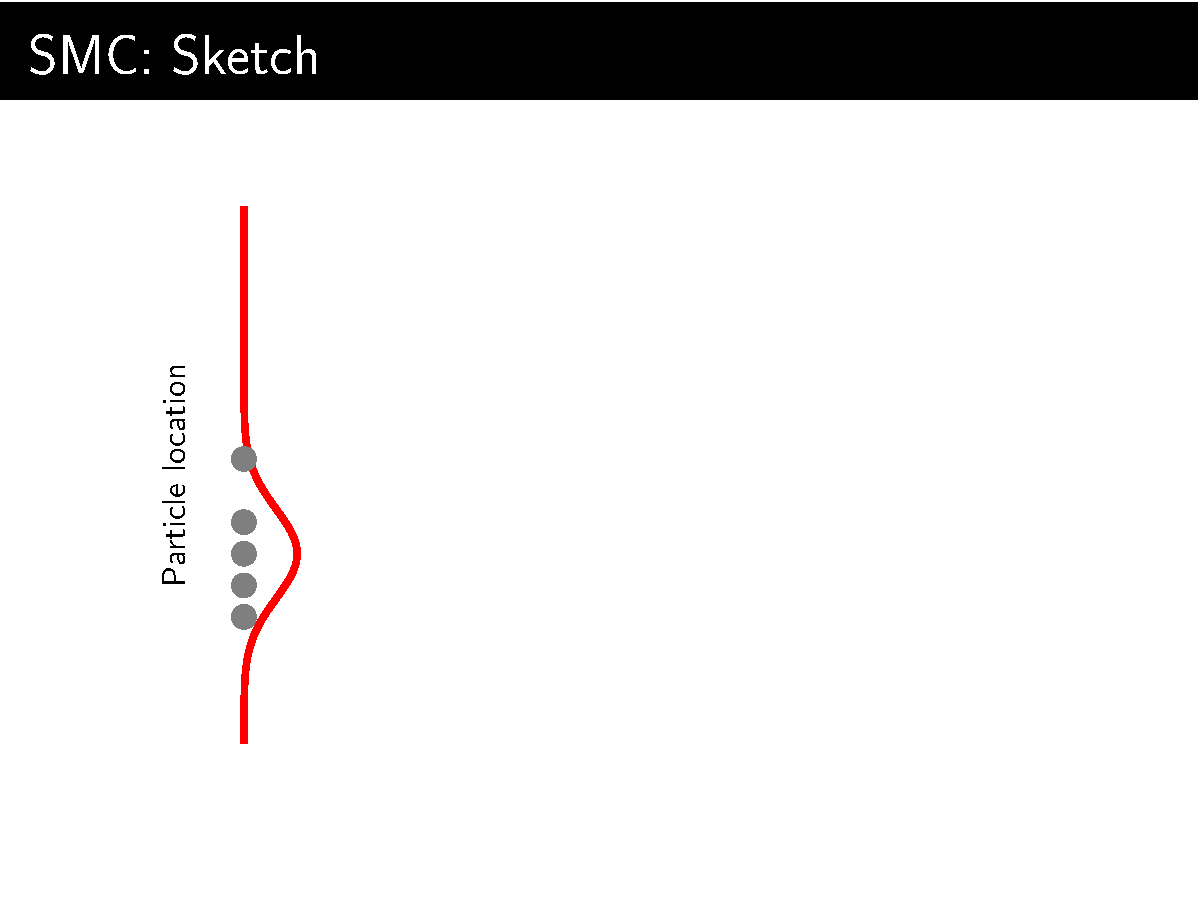
\includepdf[pages=-]{wonderful_smc_graphic_export}

%%%%%%%%%%%%%%%%%%%%%%%%%%%%%%%%%%%%%%%%%
\begin{frame}{Sequential Monte Carlo}
Given distributions $P_0, ... P_N$ such that $\frac{P_i(x, \theta)}{P_{i+1}(x, \theta)}$ is computable
\begin{itemize}
\item Sample from a tractable proposal. 
\end{itemize}

\end{frame}


%%%%%%%%%%%%%%%%%%%%%%%%%%%%%%%%%%%%%%%%%
\begin{frame}{Likelihood-free Sequential Importance Sampling}

From an earlier slide: "You need the ratios $\frac{P(x^{(i)}, \theta^{(i)})}{P(x^{(j)}, \theta^{(j)})} $ and
$ \frac{Q(x^{(j)}, \theta^{(j)})}{Q(x^{(i)}, \theta^{(i)})}$." Not (quite) true.\\

From the intro: "If you can't compute $\frac{P(x^{(i)}, \theta^{(i)})}{P(x^{(j)}, \theta^{(j)})} $, try to get the nasty part to appear in the proposal ratio."

\end{frame}

%%%%%%%%%%%%%%%%%%%%%%%%%%%%%%%%%%%%%%%%%%
%\begin{frame}{}
%
%\centering 
%	%\only<1>{\vspace*{0cm}\hspace*{0cm}\includegraphics[scale=.2]{blah.eps}}\\
%%\footnote{Graphic: blah.com}
%
%\end{frame}

%%%%%%%%%%%%%%%%%%%%%%%%%%%%%%%%%%%%%%%%%

\begin{frame}{Questions?}
Wilkinson's paper is a chapter from this book:
\bibliographystyle{splncs}
\bibliography{prelim_biblio}


\begin{center}

 %\includegraphics[ trim={0cm 0cm 0 0},clip, width = .75\textwidth]{nice_things.jpeg}
\end{center}
\end{frame}
%%%%%%%%%%%%%%%%%%%%%%%%%%%%%%%%%%%

\end{document}